\chapter{Il modello relazionale}

Il modello di base di dati relazionale è il modello più utilizzato per rappresentare ed organizzare una base dati. Questo modello si basa sul concetto matematico di relazione, ovvero la connessione tra dati è relazionata per mezzo dei valori.

Quindi, su dominio:
\[D_1, D_2, ..., D_n\]

Posso avere relazioni:

\[D_1  \times D_3\]
\[D_2  \times D_3\]
\[D_4 \times D_1\]

\section{Caratteristiche}
Questo tipo di relazione e quindi di modello ha varie caratteristiche interessanti e peculiari.

\begin{itemize}
    \item Non c'è ordine tra le righe
    \item non c'è ordine tra le colonne
    \item le righe sono tutte diverse tra loro
    \item le intestazioni sono diverse tra loro
    \item i valori contenuti nelle colonne sono dello stesso dominio.
\end{itemize}

Inoltre, come dicevamo prima la connessione tra le varie relazioni è fatta per mezzo dei valori. Sarà quindi possibile collegare i dati e creare un'informazione più estesa ed importante.


\begin{exmp}\

    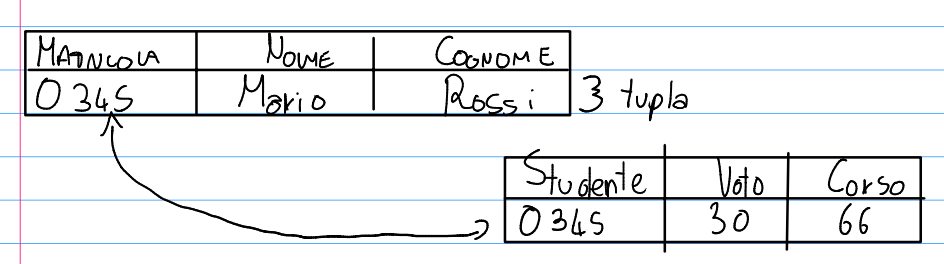
\includegraphics[width=\textwidth]{img/con_tra_rel.png}
\end{exmp}


\section{Tuple}

\begin{assioma}
Data la relazione $ R(A_1 , ..., A_n)$, una tupla è una funzione che definisce la relazione tra i vari dati. 
\end{assioma}

Le tuple vengono rappresentate come le righe delle tabelle in un database relazionale. Al singolare, una riga si chiama tupla.

Vedremo poi che una tupla è il risultato di una query, quindi non è solamente una riga della tabella se per ottenere più informazione uniamo i dati presenti in più tabelle.


%%Non chiaro
\begin{assioma}
Istanza di relazione su uno schermo $R(x)$ un insieme di tuple su $X$
\end{assioma}
%%------

\section{Valore NULL}

Il valore NULL è un valore che non fa parte del dominio, però è utile per definire dei campi in cui i dati non sono presenti.

\begin{description}
	\item[N.B.] Bisogna usare NULL con attenzione, perchè non facendo parte del dominio potrebbe dare comportamenti inattesi.
\end{description}

Per non tollerare valori nulli nel mio dominio dovrò utilizzare dei costraint.

\section{Risoluzione delle ridondanze}

Per risolvere le ridondanze, ovvero la duplicazione di dati nelle tabelle, si utilizzano i vincoli.

\section{Vincoli di integrità}

\subsection{Rigetto semantiche scorrette}
Nei database relazionali posso rigettare semantiche scorrette.

\includegraphics[width=\textwidth]{img/vincoli_di_integrità.png}

Alcuni tipi di vincoli sono supportati dal DBMS\footnote{Database management system}
Altri vincoli non sono supportati dal DBMS e vengono quindi mantenuti client side.

\subsection{Vincoli inter-relazionali}

I vincoli inter-relazionale è un vincolo che coinvolge più tabelle.

Se controllo l'integrità solo tramite vincoli di questo genere potrei però avere delle ridondanze, per questo si usa il vincolo di chiave.

\section{Vincoli di chiave}
Il vincolo di chiave dice che non posso avere tuple con i campi chiave uguali, ad esempio il codice fiscale che non può essere lo stesso per più persone.

Le chiavi verranno usate per gestire le relazioni tra tuple.

\subsection{Super-chiavi}

Un insieme $\mathbb{K}=\left\{K_1 , ..., K_n \right \} $ è una super chiave se non esistono tuple con gli stessi valori.

Una super-chiave identifica le tuple di una relazione.

Esiste infatti sempre almeno una super-chiave ed è \textbf{"tutta la tupla"}

\subsection{Chiavi}

Vedremo più in dettaglio le chiavi nel capitolo dedicato, capitolo \ref{chap:chiavi}

Una chiave è una super-chiave minimale quando:

\[\mathbb{K} \text{super-chiave è chiave} \leftrightarrow \forall k \mid k-k \text{ Non è superchiave} \]

Questa cosa va controllata che sia valida per ogni valore possibile e non solo per i valori attuali.

\begin{exmp}

Qui abbiamo un esempio delle chiavi.

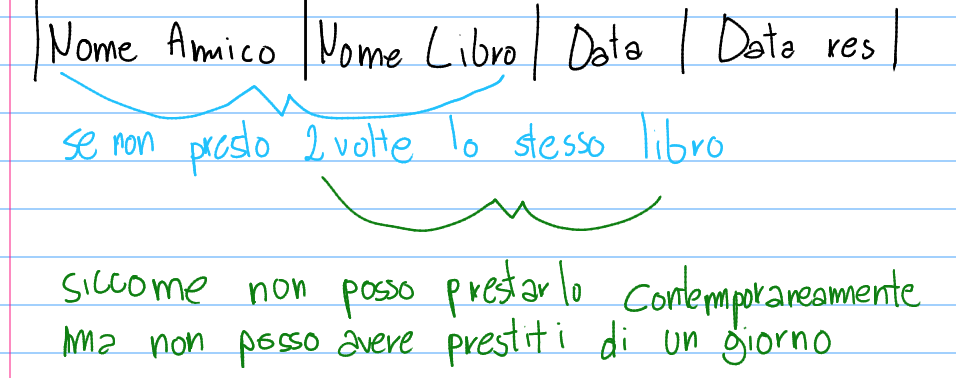
\includegraphics[width=\textwidth]{img/esempio_chiavi.png}

In questo caso infatti $(NomeAmico,NomeLibro)$ è chiave se non posso prestare allo stesso amico lo stesso libro più volte.

Nella seconda parte dell'esempio invece se $(NomeLibro,Data)$ è chiave non posso prestare lo stesso libro più volte nello stesso giorno.
\end{exmp}


